% lint-skip: 未完成ステータス（figure/table caption 未対応，人手チェック時に解消予定）
\documentclass[../../main.tex]{subfiles}
\begin{document}

\begin{flushright}
  \footnotesize\textit{【自動文字起こし・要確認】}
\end{flushright}

{\bf [解答]} 与式の左辺を$f(x)$とおくと$f(x)=0$が，2実解を持つ時
$$ a^2 - 3a + 2 \ge 0 \iff a \le 1, 2 \le a \cdots \text{(1)} $$

以下，$ay \ge 3(x-\beta)$ \dots (2) について考える．まず，$ay=3(x-\beta)$が$(\beta, 0)$を通るから$\beta>0$が必要．これは(1)のもとで
$$
\begin{cases} \text{端点} f(0) > 0 \\ \text{軸} \dfrac{3}{2}a > 0
\end{cases} \iff
\begin{cases} 3a-2 > 0 \\ a > 0
\end{cases} \iff a > \dfrac{2}{3} \cdots \text{(3)} $$
だから，(3)が条件．このもとで，
\paragraph{(2)}

$\iff y \ge \dfrac{3}{a}(x-\beta)$
より条件は
$\dfrac{3}{a} > 1 \iff 3 > a \cdots \text{(4)}$

\begin{figure}[htb]
  \centering
  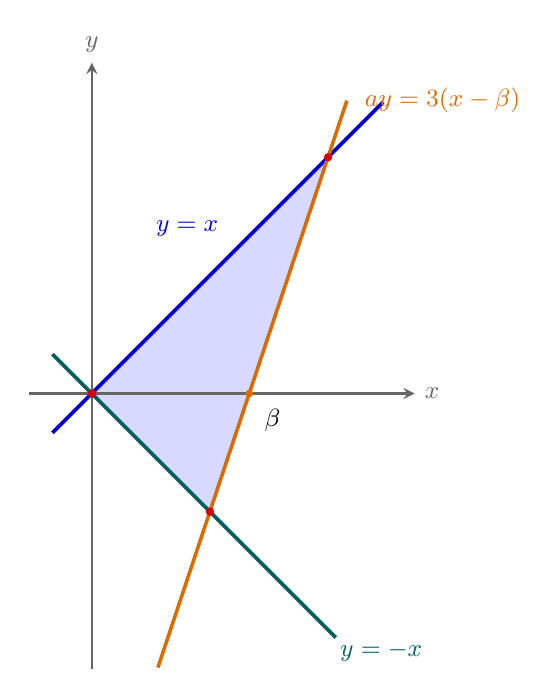
\begin{tikzpicture}[x=2cm, y=2cm, >=stealth,
    every node/.style={font=\small}]
    % Example: a=1 and beta=1, so the third boundary is y=3(x-1).
    \fill[blue!15] (0,0) -- (1.5,1.5) -- (0.75,-0.75) -- cycle;
    \draw[->, thick, gray!80!black] (-0.4,0) -- (2.05,0)
    node[right] {$x$};
    \draw[->, thick, gray!80!black] (0,-1.75) -- (0,2.1)
    node[above] {$y$};
    \draw[line width=1.3pt, blue!85!black]
    (-0.25,-0.25) -- (1.85,1.85);
    \draw[line width=1.3pt, teal!75!black]
    (-0.25,0.25) -- (1.55,-1.55);
    \draw[line width=1.3pt, orange!85!black]
    (0.42,-1.74) -- (1.62,1.86);
    \fill[red!85!black] (0,0) circle (1.5pt);
    \fill[red!85!black] (1.5,1.5) circle (1.5pt);
    \fill[red!85!black] (0.75,-0.75) circle (1.5pt);
    \fill[orange!85!black] (1,0) circle (1.4pt);
    \node[above left=2pt, blue!85!black] at (0.9,0.9) {$y=x$};
    \node[below right=2pt, teal!75!black] at (1.48,-1.48)
    {$y=-x$};
    \node[right=3pt, orange!85!black] at (1.62,1.86)
    {$ay=3(x-\beta)$};
    \node[below right=2pt] at (1,0) {$\beta$};
  \end{tikzpicture}
  \caption{3本の直線に囲まれる三角形領域（$a=\beta=1$ の例）}
\end{figure}

(1), (3), (4) から
$$ \dfrac{2}{3} < a \le 1, \quad 2 \le a < 3 $$

\end{document}
